\begin{pages}
    \begin{Rightside}
    \selectlanguage{greek}
        \beginnumbering
        \pstart[
        			\chapter{Ὁ ἐκ τοῦ οὐρανοῦ πεπτωκὼς ἀστήρ}
        			\markboth{The Star Having Fallen from Heaven}
				]
		Καὶ ὁ πέμπτος ἄγγελος ἐσάλπισεν· καὶ εἶδον ἀστέρα ἐκ τοῦ οὐρανοῦ πεπτωκότα εἰς τὴν γῆν, καὶ ἐδόθη αὐτῷ ἡ κλεὶς τοῦ φρέατος τῆς ἀβύσσου. καὶ ἤνοιξεν τὸ φρέαρ τῆς ἀβύσσου· καὶ ἀνέβη καπνὸς ἐκ τοῦ φρέατος ὡς καπνὸς καμίνου μεγάλης, καὶ ἐσκοτώθη ὁ ἥλιος καὶ ὁ ἀὴρ ἐκ τοῦ καπνοῦ τοῦ φρέατος. 
		\pend
		\pstart
		καὶ ἐκ τοῦ καπνοῦ ἐξῆλθον ἀκρίδες εἰς τὴν γῆν, καὶ ἐδόθη αὐτοῖς ἐξουσία ὡς ἔχουσιν ἐξουσίαν οἱ σκορπίοι τῆς γῆς. καὶ ἐρρέθη αὐτοῖς ἵνα μὴ ἀδικήσουσιν τὸν χόρτον τῆς γῆς οὐδὲ πᾶν χλωρὸν οὐδὲ πᾶν δένδρον, εἰ μὴ τοὺς ἀνθρώπους οἵτινες οὐκ ἔχουσιν τὴν σφραγῖδα τοῦ Θεοῦ ἐπὶ τῶν μετώπων. 
		\pend
		\pstart
		καὶ ἐδόθη αὐτοῖς ἵνα μὴ ἀποκτείνωσιν αὐτούς, ἀλλ’ ἵνα βασανισθήσονται μῆνας πέντε· καὶ ὁ βασανισμὸς αὐτῶν ὡς βασανισμὸς σκορπίου, ὅταν παίσῃ ἄνθρωπον. καὶ ἐν ταῖς ἡμέραις ἐκείναις ζητήσουσιν οἱ ἄνθρωποι τὸν θάνατον καὶ οὐ μὴ εὑρήσουσιν αὐτόν, καὶ ἐπιθυμήσουσιν ἀποθανεῖν καὶ φεύγει ὁ θάνατος ἀπ’ αὐτῶν. 
		\pend
		\pstart
		καὶ τὰ ὁμοιώματα τῶν ἀκρίδων ὅμοιοι ἵπποις ἡτοιμασμένοις εἰς πόλεμον, καὶ ἐπὶ τὰς κεφαλὰς αὐτῶν ὡς στέφανοι ὅμοιοι χρυσῷ, καὶ τὰ πρόσωπα αὐτῶν ὡς πρόσωπα ἀνθρώπων, καὶ εἶχαν τρίχας ὡς τρίχας γυναικῶν, καὶ οἱ ὀδόντες αὐτῶν ὡς λεόντων ἦσαν, καὶ εἶχον θώρακας ὡς θώρακας σιδηροῦς, καὶ ἡ φωνὴ τῶν πτερύγων αὐτῶν ὡς φωνὴ ἁρμάτων ἵππων πολλῶν τρεχόντων εἰς πόλεμον. 
		\pend
		\pstart
		καὶ ἔχουσιν οὐρὰς ὁμοίας σκορπίοις καὶ κέντρα, καὶ ἐν ταῖς οὐραῖς αὐτῶν ἡ ἐξουσία αὐτῶν ἀδικῆσαι τοὺς ἀνθρώπους μῆνας πέντε. ἔχουσιν ἐπ’ αὐτῶν βασιλέα τὸν ἄγγελον τῆς ἀβύσσου, ὄνομα αὐτῷ Ἑβραϊστί Ἀβαδδών καὶ ἐν τῇ Ἑλληνικῇ ὄνομα ἔχει Ἀπολλύων. Ἡ Οὐαὶ ἡ μία ἀπῆλθεν· ἰδοὺ ἔρχεται ἔτι δύο Οὐαὶ μετὰ ταῦτα.
		\pend
		\pstart
		Καὶ ὁ ἕκτος ἄγγελος ἐσάλπισεν· καὶ ἤκουσα φωνὴν μίαν ἐκ τῶν τεσσάρων κεράτων τοῦ θυσιαστηρίου τοῦ χρυσοῦ τοῦ ἐνώπιον τοῦ Θεοῦ, λέγοντα τῷ ἕκτῳ ἀγγέλῳ, ὁ ἔχων τὴν σάλπιγγα Λῦσον τοὺς τέσσαρας ἀγγέλους τοὺς δεδεμένους ἐπὶ τῷ ποταμῷ τῷ μεγάλῳ Εὐφράτῃ. καὶ ἐλύθησαν οἱ τέσσαρες ἄγγελοι οἱ ἡτοιμασμένοι εἰς τὴν ὥραν καὶ ἡμέραν καὶ μῆνα καὶ ἐνιαυτόν, ἵνα ἀποκτείνωσιν τὸ τρίτον τῶν ἀνθρώπων. καὶ ὁ ἀριθμὸς τῶν στρατευμάτων τοῦ ἱππικοῦ δισμυριάδες μυριάδων· ἤκουσα τὸν ἀριθμὸν αὐτῶν. 
		\pend
		\pstart
		καὶ οὕτως εἶδον τοὺς ἵππους ἐν τῇ ὁράσει καὶ τοὺς καθημένους ἐπ’ αὐτῶν, ἔχοντας θώρακας πυρίνους καὶ ὑακινθίνους καὶ θειώδεις· καὶ αἱ κεφαλαὶ τῶν ἵππων ὡς κεφαλαὶ λεόντων, καὶ ἐκ τῶν στομάτων αὐτῶν ἐκπορεύεται πῦρ καὶ καπνὸς καὶ θεῖον. 
		\pend
		\pstart
		ἀπὸ τῶν τριῶν πληγῶν τούτων ἀπεκτάνθησαν τὸ τρίτον τῶν ἀνθρώπων, ἐκ τοῦ πυρὸς καὶ τοῦ καπνοῦ καὶ τοῦ θείου τοῦ ἐκπορευομένου ἐκ τῶν στομάτων αὐτῶν. ἡ γὰρ ἐξουσία τῶν ἵππων ἐν τῷ στόματι αὐτῶν ἐστιν καὶ ἐν ταῖς οὐραῖς αὐτῶν· αἱ γὰρ οὐραὶ αὐτῶν ὅμοιαι ὄφεσιν, ἔχουσαι κεφαλάς, καὶ ἐν αὐταῖς ἀδικοῦσιν.
		\pend
		\pstart
		καὶ οἱ λοιποὶ τῶν ἀνθρώπων, οἳ οὐκ ἀπεκτάνθησαν ἐν ταῖς πληγαῖς ταύταις, οὐδὲ μετενόησαν ἐκ τῶν ἔργων τῶν χειρῶν αὐτῶν, ἵνα μὴ προσκυνήσουσιν τὰ δαιμόνια καὶ τὰ εἴδωλα τὰ χρυσᾶ καὶ τὰ ἀργυρᾶ καὶ τὰ χαλκᾶ καὶ τὰ λίθινα καὶ τὰ ξύλινα, ἃ οὔτε βλέπειν δύνανται οὔτε ἀκούειν οὔτε περιπατεῖν, καὶ οὐ μετενόησαν ἐκ τῶν φόνων αὐτῶν οὔτε ἐκ τῶν φαρμακιῶν αὐτῶν οὔτε ἐκ τῆς πορνείας αὐτῶν οὔτε ἐκ τῶν κλεμμάτων αὐτῶν.
		\pend
        \endnumbering
    \end{Rightside}
    \begin{Leftside}
        \beginnumbering
        \pstart[
        			\chapter{The Star Having Fallen from Heaven}
				]
		And the fifth angel sounded (his trumpet). And I saw a star having fallen from Heaven (down on)to Earth and the key to the well of the abyss (bottomless pit) was given to him; and he opened the well of the abyss. And there came forth a great smoke from the well, like (the) smoke of a great furnace; and the Sun and the air were darkened (overshadowed) from (because of, through) the smoke of the well. 
		\pend
		\pstart
		And from the smoke there emerged grasshoppers (and they went out) upon the Earth, and they were given the (same) authority as the authority of the scorpions of the Earth. And they were told to not harm the grass of the Earth, nor any (all) green things nor any (all) tree, except for (they were allowed to harm) the humans who do not have the seal of God upon their foreheads. 
		\pend
		\pstart
		And it was given to them (the grasshoppers) so that they might not kill them (the unsealed), but so that they shall be tormented for five months; and their torment (was) like the torment of a scorpion when he strikes a person. And in those days, men will seek Death but shall not find him; they will yearn to die, but 	Death flees from them. 
		\pend
		\pstart
		And the appearance of the grasshoppers was like that of horses preparing (themselves to go) into battle and upon their heads are (placed things that look like) crowns — (which are in appearance) like gold — and their faces are like the faces of men; and they have a mane (hairs) like the hair of women and their teeth were like (those) of lions. And they had breastplates (which looked) like iron breastplates and the voice (sound) of the their wings (was) as the voice of a chariot of horses marching into battle (going to war). 
		\pend
		\pstart
		And they have tails like (those of) scorpions and (they also have) stings (at the end of their tails?). And in their tails (is) the authority to hurt (all) the humans for five months. And they have (sitting?) upon them a king — the angel of the abyss — whose name, in Hebrew, is Abaddon and in the Greek language he has the name Apollyon. The first Woe departed — (but) look! There are coming yet two more Woes hereafter. 
		\pend
		\pstart
		And the sixth angel sounded (his trumpet). And I heard a voice (emerging) from the four horns of the golden altar before God telling the sixth angel — the one holding the trumpet —, “Release the four angels, the ones that are bound to (in) the great river Euphrates.” And the four angels were released, namely the ones who prepared (themselves) for the hour and the day and the year (during which) they might kill a third of the humans. And the number of the army of horsemen was two-hundred thousand thousands; I heard their number.
		\pend
		\pstart
		And thus (in this manner) I saw the horses in the vision and (I also saw those those) who sit upon them, having fiery, hyacinthine (purple) and brimstone-like (colour of sulfur) breastplates. And the heads of the horses (were) as the heads of lions, and from their mouths sprang forth fire and smoke and brimstone (sulfur).
		\pend 
		\pstart
		A third of the human (race) died from these three plagues — from the fire, and the smoke and the brimstone (sulfur) which sprang forth from their mouths. For the power (authority) of the horses is (placed) in(side) their mouth and in(side) their tails. For their tails are like snakes with (having) heads — and in (using them) they (do) harm. 
		\pend
		\pstart
		And the remaining humans, those who did neither die from those plagues nor repented of the works of their (own) hands that they should not worship demons and golden, silver, copper, wooden or stone idols — who (the idols) can neither see nor listen nor walk about; and (those humans who) neither repented of their (committed) murders nor of their drug-usage (magic, sorcery) nor of their sexual immorality nor of their (committed) thefts. 
		\pend
        \endnumbering
    \end{Leftside}

\end{pages} 
\Pages

\clearpage
\thispagestyle{empty}
\null\vfill
\settowidth\longest{\huge\itshape […] and when I turned around I saw}
\begin{center}
\parbox{\longest}{%
  \raggedright{\huge\itshape%
    ``And I saw a star having fallen from Heaven (down on)to Earth […]'' \par\bigskip
  }
  \raggedleft\Large\MakeUppercase{``And I saw a Star fall from Heaven'' — John Henry Stock, 1902}\par%
}
\vfill\vfill
\clearpage\newpage
\end{center}
\newpage
\thispagestyle{empty}
\begin{center}
	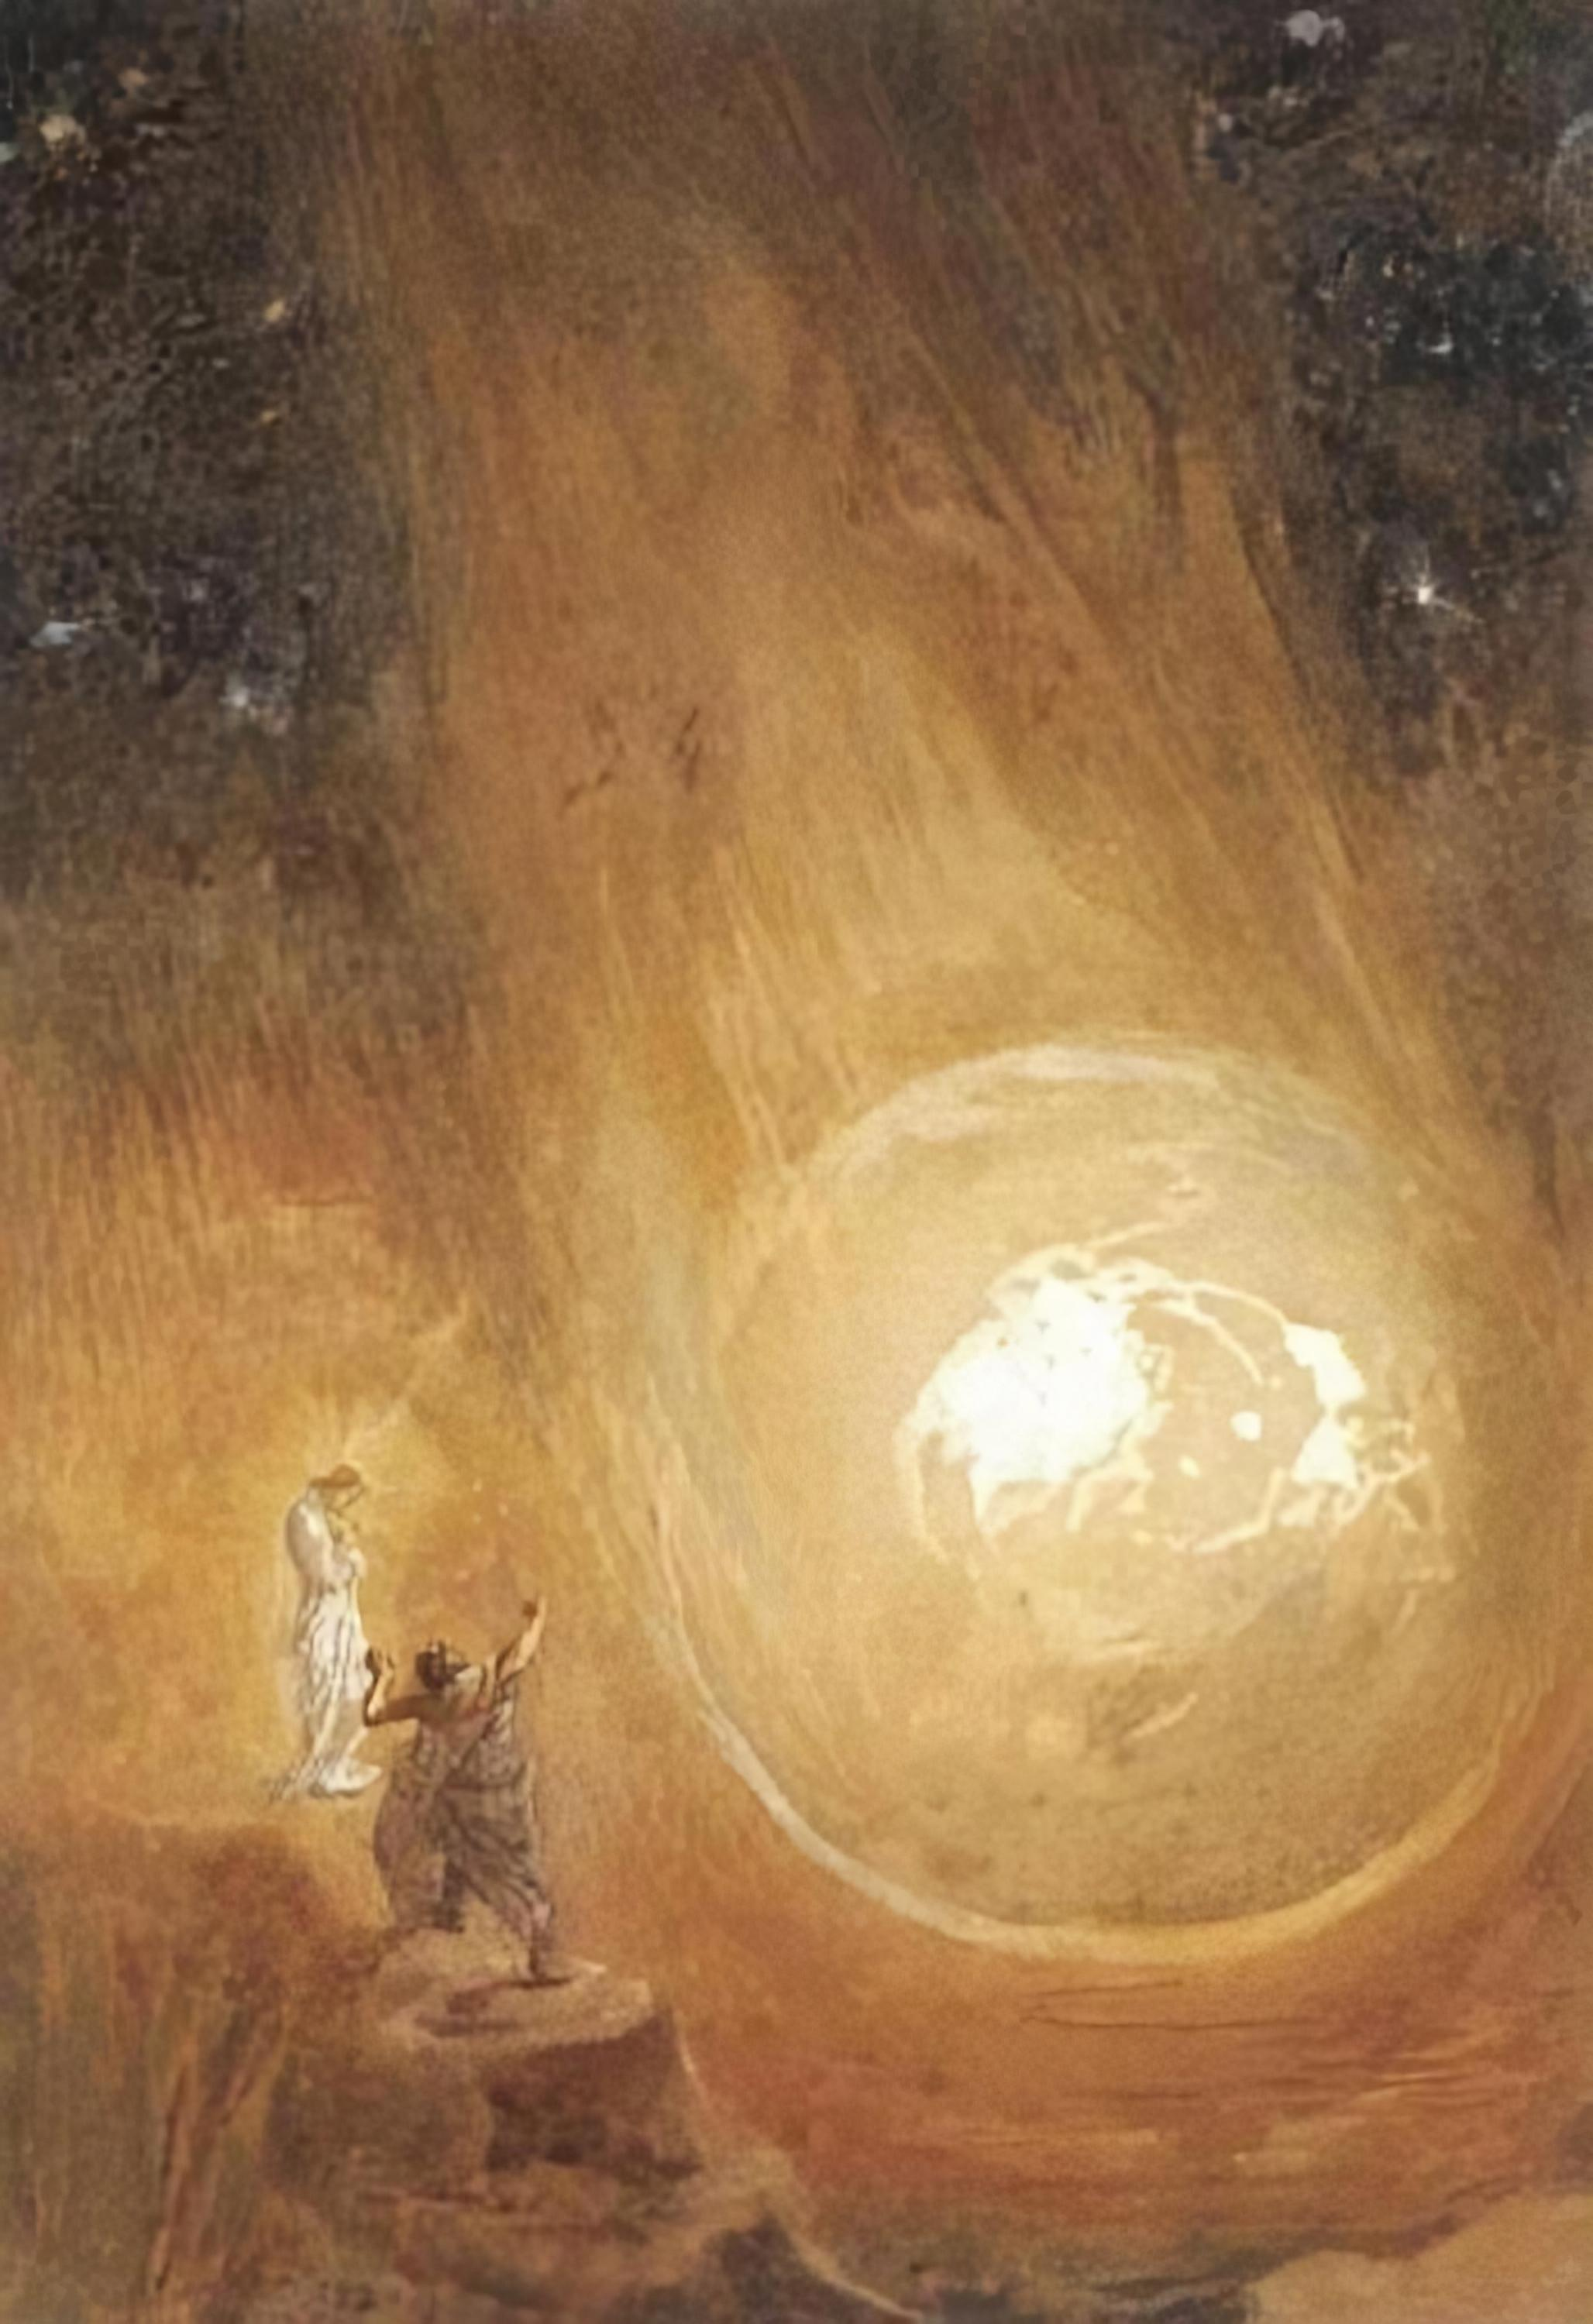
\includegraphics[width=0.96\textwidth]{images/illustrations/stockfallenstar}
\end{center}